\documentclass[a0paper,portrait]{baposter}

\usepackage{relsize}		% For \smaller
\usepackage{url}			% For \url
\usepackage{multirow}
\usepackage{multicol}
\usepackage[utf8]{inputenc}
% a font close to that chosen by Elsevier
\usepackage[bitstream-charter]{mathdesign}
% for accentuated characters
\usepackage[T1]{fontenc}
%%% Global Settings %%%%%%%%%%%%%%%%%%%%%%%%%%%%%%%%%%%%%%%%%%%%%%%%%%%%%%%%%%%

\graphicspath{{figures/}}	% Root directory of the pictures 
\tracingstats=2			% Enabled LaTeX logging with conditionals

%%% Color Definitions %%%%%%%%%%%%%%%%%%%%%%%%%%%%%%%%%%%%%%%%%%%%%%%%%%%%%%%%%

\definecolor{bordercol}{RGB}{40,40,40}
\definecolor{headercol1}{RGB}{186,215,230}
\definecolor{headercol2}{RGB}{255,255,255}
\definecolor{headerfontcol}{RGB}{0,0,0}
\definecolor{boxcolor}{RGB}{255,255,255}

%%%%%%%%%%%%%%%%%%%%%%%%%%%%%%%%%%%%%%%%%%%%%%%%%%%%%%%%%%%%%%%%%%%%%%%%%%%%%%%%
%%% Utility functions %%%%%%%%%%%%%%%%%%%%%%%%%%%%%%%%%%%%%%%%%%%%%%%%%%%%%%%%%%

%%% Save space in lists. Use this after the opening of the list %%%%%%%%%%%%%%%%
\newcommand{\compresslist}{
	\setlength{\itemsep}{1pt}
	\setlength{\parskip}{0pt}
	\setlength{\parsep}{0pt}
}
\DeclareTextSymbol{\degr}{T1}{6}
%%%%%%%%%%%%%%%%%%%%%%%%%%%%%%%%%%%%%%%%%%%%%%%%%%%%%%%%%%%%%%%%%%%%%%%%%%%%%%%
%%% Document Start %%%%%%%%%%%%%%%%%%%%%%%%%%%%%%%%%%%%%%%%%%%%%%%%%%%%%%%%%%%%
%%%%%%%%%%%%%%%%%%%%%%%%%%%%%%%%%%%%%%%%%%%%%%%%%%%%%%%%%%%%%%%%%%%%%%%%%%%%%%%
\begin{document}

%----------------------------------------------------------------------------------------
%	POSTER HEADER 
%----------------------------------------------------------------------------------------
\begin{poster}{
	grid=false,
	% Option is left on true though the eyecatcher is not used. The reason is
	% that we have a bit nicer looking title and author formatting in the headercol
	% this way
	%eyecatcher=false, 
	borderColor=bordercol,
	headerColorOne=headercol1,
	headerColorTwo=headercol2,
	headerFontColor=headerfontcol,
	% Only simple background color used, no shading, so boxColorTwo isn't necessary
	boxColorOne=boxcolor,
	headershape=smallrounded,
	headerfont=\Large\sf\bf,
	textborder=roundedsmall,
	background=none,
	headerborder=open,
    boxshade=plain,
    columns= 4
}
{}
{
Measuring the contact area by SPM imaging
}
{
{\color{red}L. Charleux}, {\color{green}\underline{V. Keryvin}}, {\color{cyan}J.-P. Guin, M. Nivard, J.-C. Sangleb\oe uf}, {\color{blue}Y. Yokoyama}

\begin{small}
{\color{red}Univ. Savoie Mont Blanc (France)}, {\color{green}Univ. Bretagne Sud (France)}, {\color{cyan}Univ. Rennes 1 (France)}, {\color{blue}Tohoku Univ. Sendai (Japan)}
\end{small}

}
{

%
%
\includegraphics[height = 1cm]{symme} 
\includegraphics[height= 1cm]{limatb} 
\includegraphics[height = 1cm]{ipr}

}

%\headerbox{Abstract}{name=abstract,column=2, span = 2,row=0}
%{
%The determination of the contact area is a key step to derive mechanical properties such as hardness or an elastic modulus by instrumented indentation testing. Two families of procedures are dedicated to extracting this area: on the one hand, \textit{post mortem} measurements that require residual imprint imaging, and on the other hand, direct methods that only rely on the load \textit{vs.} the penetration depth curve. With the development of built-in scanning probe microscopy imaging capabilities such as atomic force microscopy and indentation tip scanning probe microscopy, last generation indentation devices have made systematic residual imprint imaging much faster and more reliable. In this paper, a new \textit{post mortem} method is introduced and further compared to three existing classical direct methods by means of a numerical and experimental benchmark covering a large range of materials. It is shown that the new method systematically leads to lower error levels regardless of the type of material. Pros and cons of the new method \textit{vs.} direct methods are also discussed, demonstrating its efficiency in easily extracting mechanical properties with an enhanced confidence. 
%}


\headerbox{Indentation + SPM imaging}{name=materials,column=0, span = 2,row=0}
{

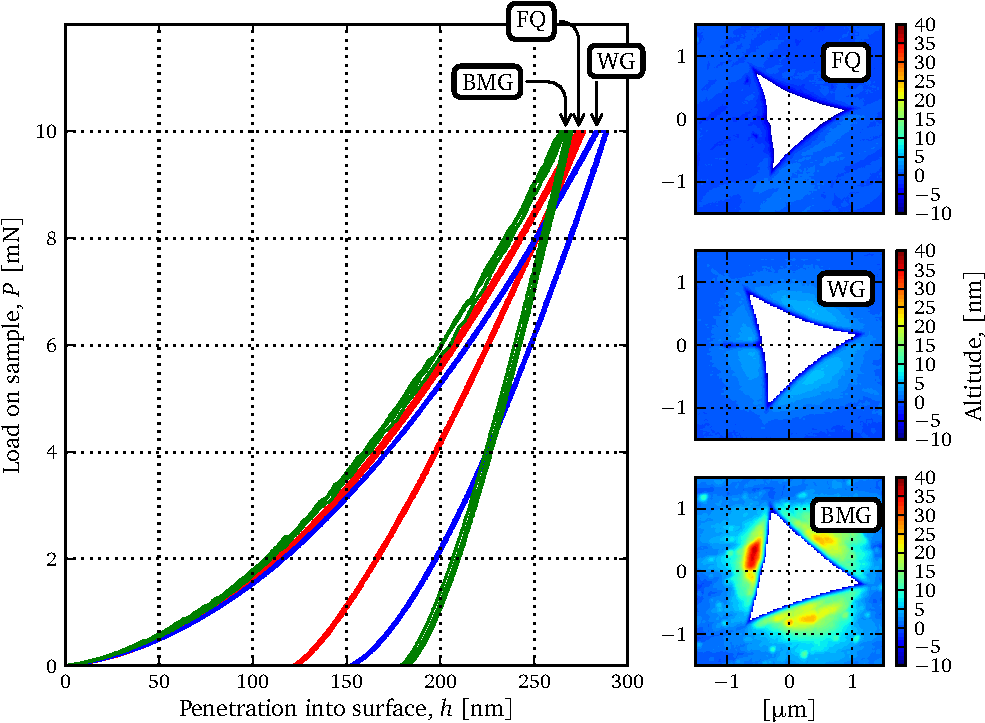
\includegraphics[width=\linewidth]{figure_3}

}


\headerbox{Measuring the contact area $A_c$}{ name=method,column=2, span = 2,row=0}
{
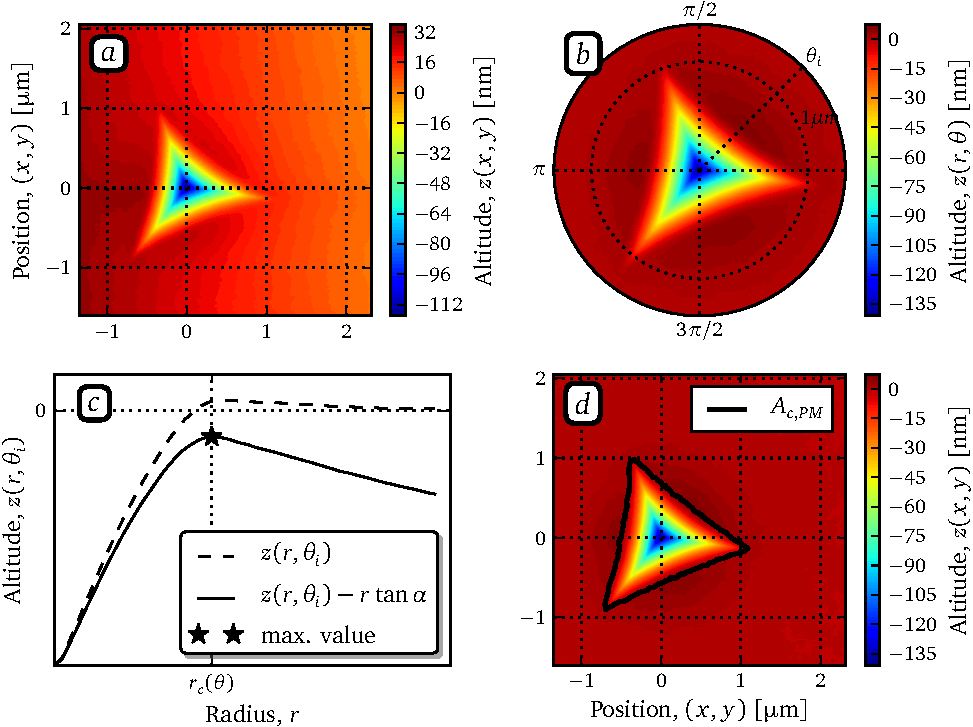
\includegraphics[width=\linewidth]{figure_4}
}

\headerbox{The role of $\alpha$}{below= materials, name=alpha,column=0, span = 2,row=0}
{
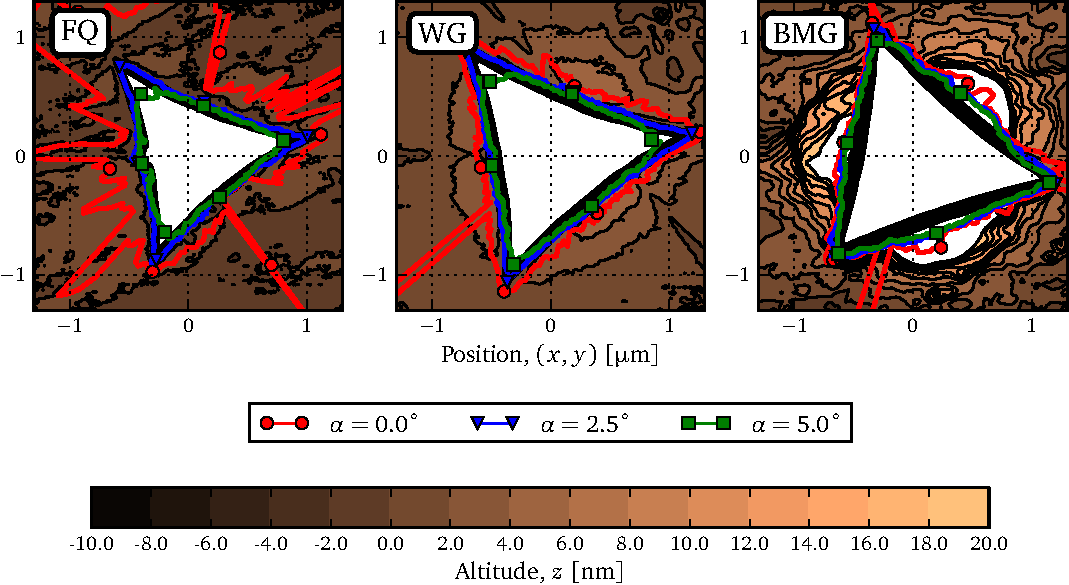
\includegraphics[width=\linewidth]{figure_8}
}
%
%\headerbox{Numerical Benchmark}{below = method, name=num_benchmark,column=0, span = 2,row=0}
%{
%
%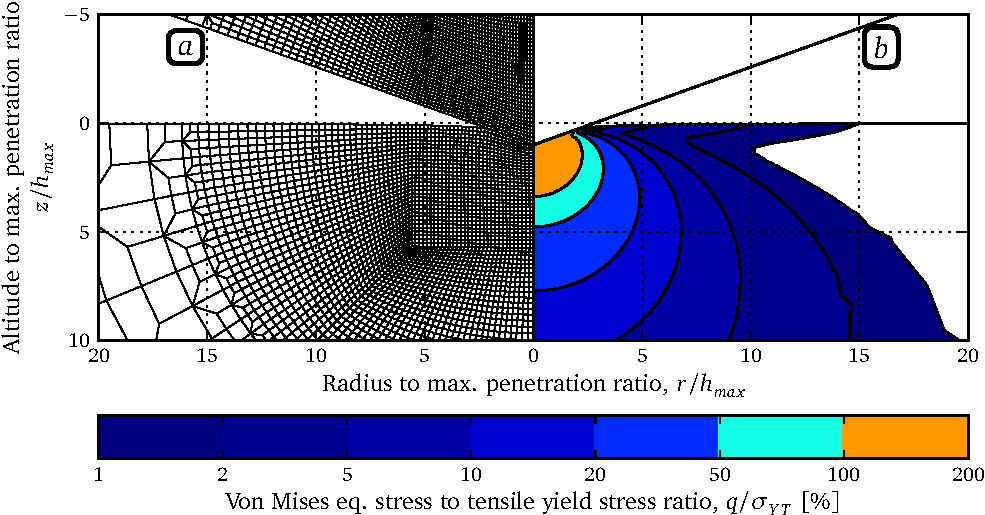
\includegraphics[width=\linewidth]{figure_2}
%
%}
%
%
%
%
\headerbox{Numerical benchmark}{below =method, name=num_results,column=2, span = 2,row=0}
{
\begin{center}
Hollomon 
\end{center}
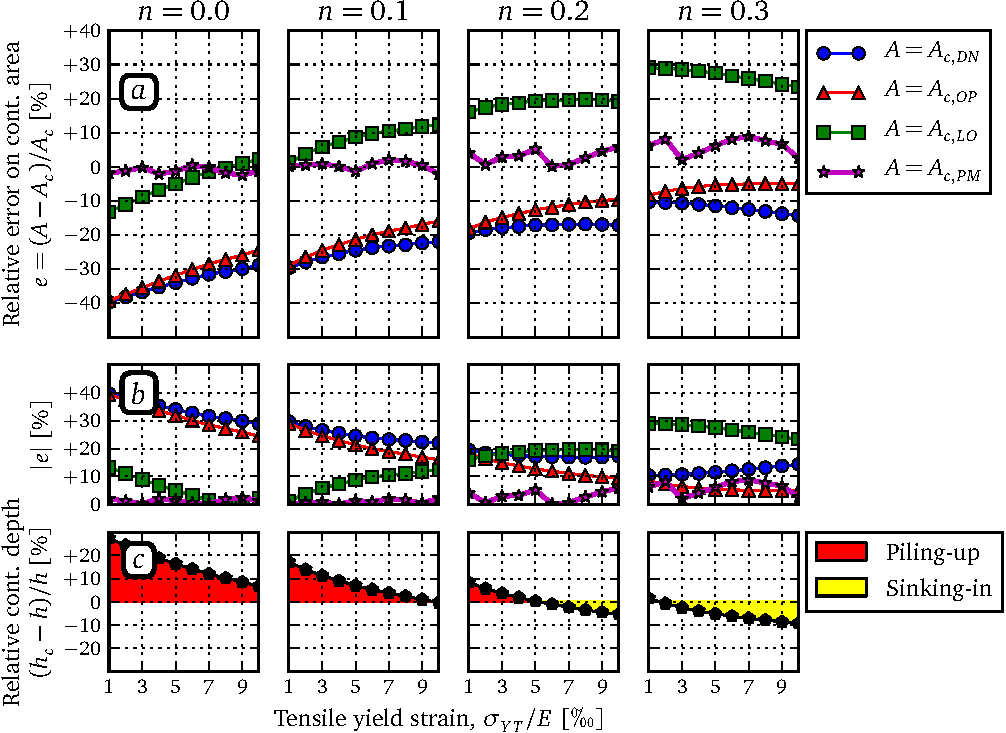
\includegraphics[width=\linewidth]{figure_5}\\
\begin{center}
Drucker-Prager
\end{center}
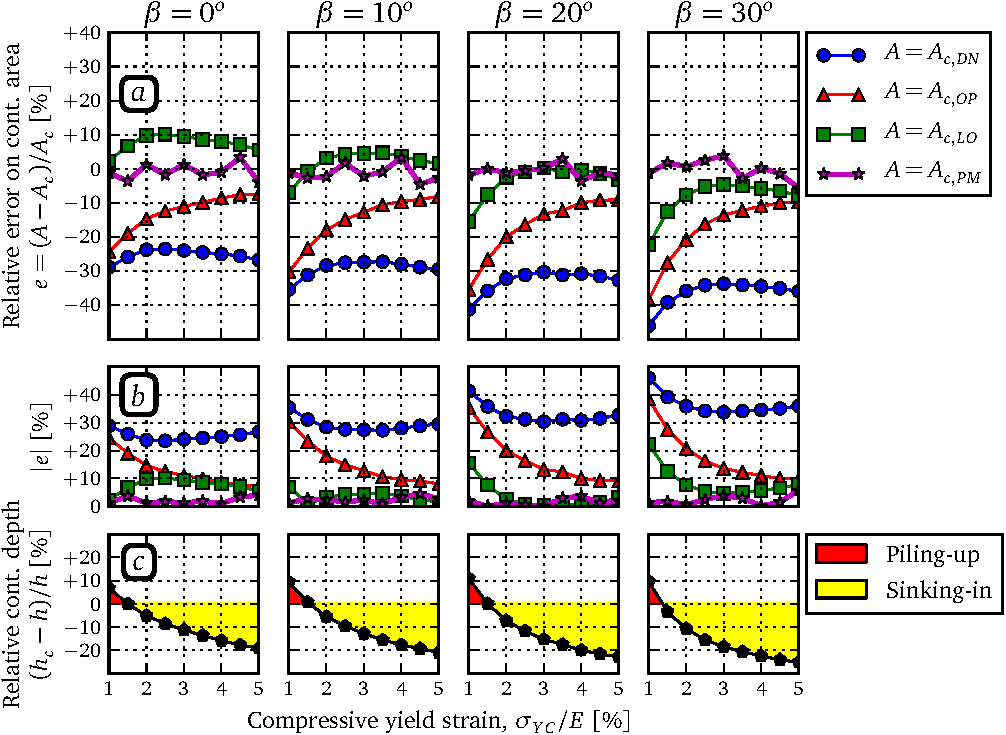
\includegraphics[width=\linewidth]{figure_6}

}
%
\headerbox{Experimental benchmark}{below =alpha, name=exp_benchmark,column=0, span = 2,row=0}
{

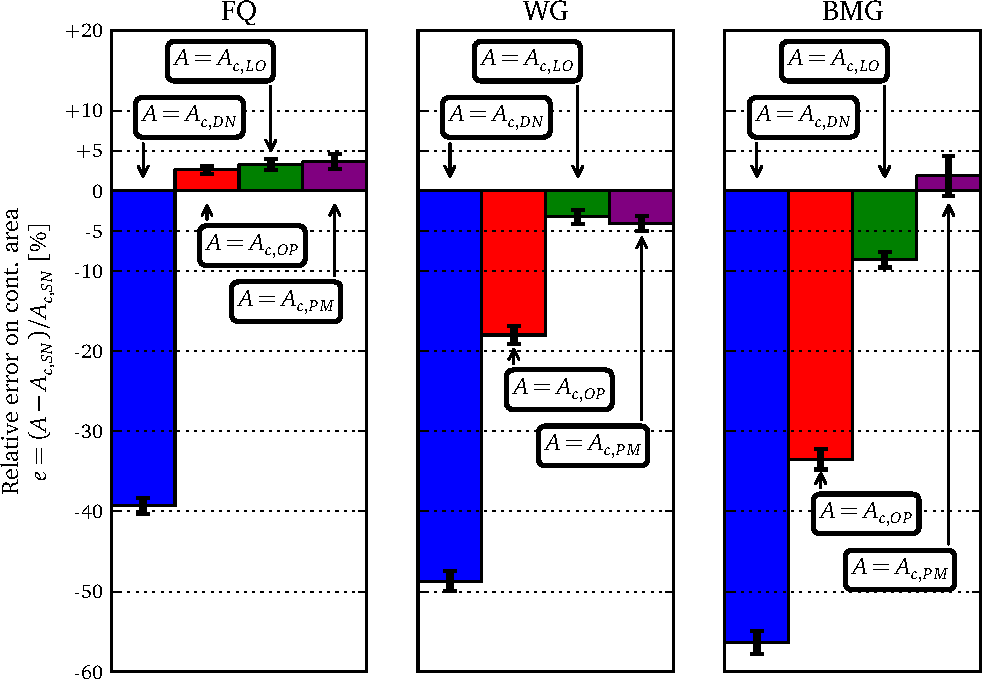
\includegraphics[width=\linewidth]{figure_7}


}
\headerbox{References}{below =exp_benchmark, name=refs,column=0, span = 2,row=0}
{
\begin{itemize}
\item \url{https://github.com/lcharleux/spym}
\item L. Charleux, V. Keryvin, M. Nivard, J.-P. Guin, J.-C. Sanglebœuf, and Y. Yokoyama, “A method for measuring the contact area in instrumented indentation testing by tip scanning probe microscopy imaging” Acta Mater., vol. 70, pp. 249–258,2014.
\end{itemize}



}

\end{poster}



%%----------------------------------------------------------------------------------------
%%	ABSTRACT
%%----------------------------------------------------------------------------------------
%
%\color{Navy} % Navy color for the abstract
%
%\begin{abstract}
%The determination of the contact area is a key step to derive mechanical properties such as hardness or an elastic modulus by instrumented indentation testing. Two families of procedures are dedicated to extracting this area: on the one hand, \textit{post mortem} measurements that require residual imprint imaging, and on the other hand, direct methods that only rely on the load \textit{vs.} the penetration depth curve. With the development of built-in scanning probe microscopy imaging capabilities such as atomic force microscopy and indentation tip scanning probe microscopy, last generation indentation devices have made systematic residual imprint imaging much faster and more reliable. In this paper, a new \textit{post mortem} method is introduced and further compared to three existing classical direct methods by means of a numerical and experimental benchmark covering a large range of materials. It is shown that the new method systematically leads to lower error levels regardless of the type of material. Pros and cons of the new method \textit{vs.} direct methods are also discussed, demonstrating its efficiency in easily extracting mechanical properties with an enhanced confidence. 
%\end{abstract}
%%----------------------------------------------------------------------------------------
%%	INTRODUCTION
%%----------------------------------------------------------------------------------------
%
%\color{Black} % SaddleBrown color for the introduction
%\section*{Introduction}
%
%
%\begin{center}
%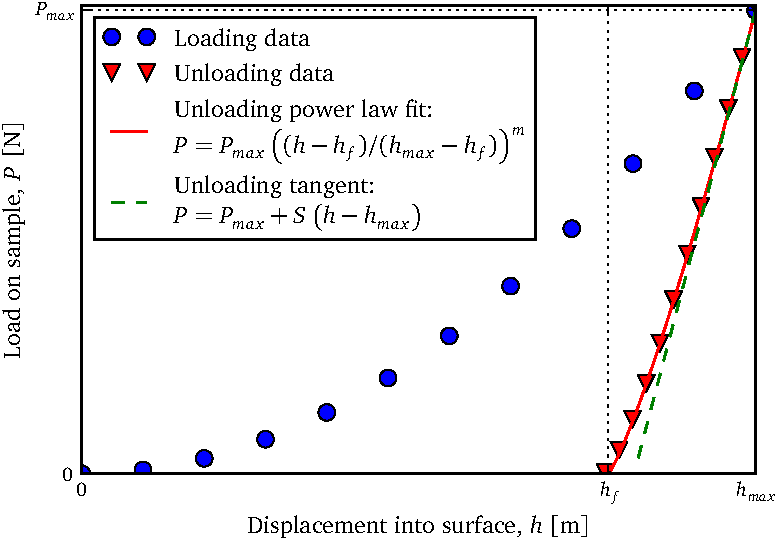
\includegraphics[width = 20cm]{figure_1}
%\captionof{figure}{Typical sharp indentation load on sample \textit{vs.} displacement into surface curve. The test is split into a loading step and an unloading step. The experimental curve generally also includes an holding step which is not represented in this case. The contact stiffness $S$ is the unloading step's initial slope. However, the direct determination of $S$ \textit{via} the upper part of the step is unreliable as it uses only a small part of the curve. For increased accuracy, the whole step is systematically fitted by a power law function which is used to compute back the contact stiffness $S$ as initially recommended in \cite{ISI:000222316100002}.}
%\end{center}
%
%
%
%\begin{center}
%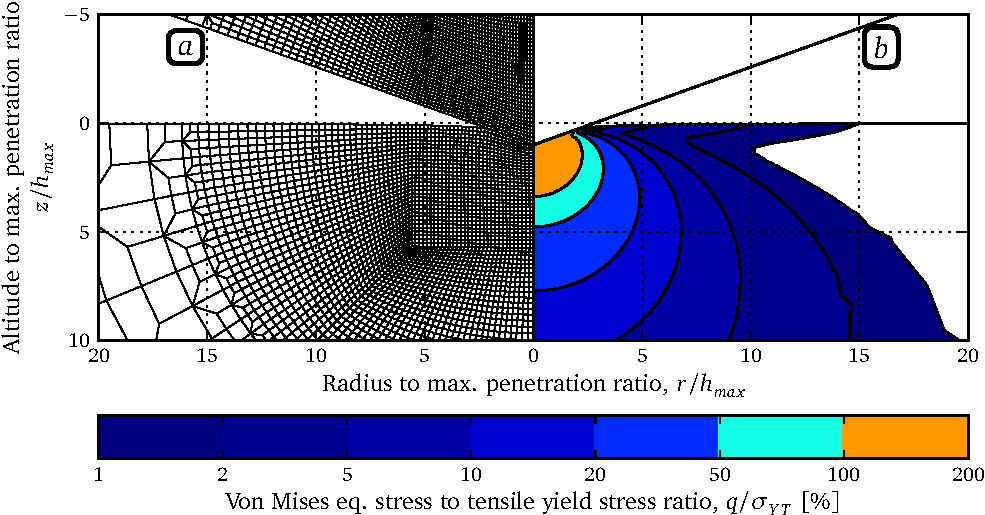
\includegraphics[width = 20cm]{figure_2}
%\captionof{figure}{Representation of the 2D axisymmetric FEM model including a rigid conical indenter and a deformable elastic-plastic sample. In this particular case, the sample's material is based on CE1 ($\sigma_{YT}/E = 0.07$, $n = 0.3$). The model is represented at maximum penetration into surface $h_{max}$.  (\textbf{a}) The deformed mesh is plotted showing the finely meshed zone containing the contact zone and most of the plastic zone. This zone is initially filled with square shaped elements. The mesh is gradually coarsened away from the contact zone. The whole mesh is not represented since its total size is about $10^3$ times the size of the finely mesh zone. (\textbf{b}) The gradient represents the ratio of the von Mises equivalent stress in tension $q$ to the tensile yield stress $\sigma_{YT}$ with the corresponding scale given by the bottom color bar.}
%
%\end{center}
%
%
%
%\begin{center}
%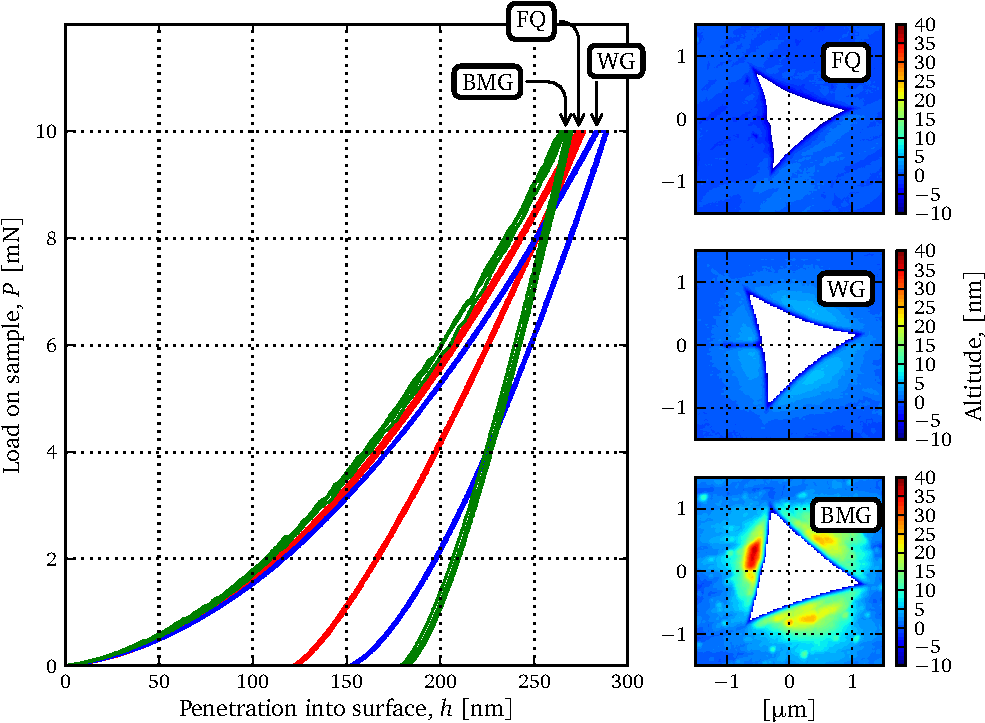
\includegraphics[width = 20cm]{figure_3}
%\captionof{figure}{Representation of the experimental tests carried out on the three selected materials FQ, WG and BMG (Four tests per sample). (\textbf{Left}) The load \textit{vs.} displacement into surface $(P,h)$ curves are plotted. The three loading steps are rather similar while the unloading steps are very different. The FQ exhibits very high elastic recovery while the BMG has a low one. (\textbf{Right}) ITSPM of one of the four tests is plotted for each material. Altitudes below 10 nm are masked in order to emphasize the shape and size of the residual piling-up. There is no visible residual piling-up on FQ, a low altitude circular one on WG and a higher altitude one with summits on the faces on BMG. These observations justify the choice of the three selected materials as they cover all possible contact geometries.}
%
%\end{center}
%
%
%
%
%\begin{center}
%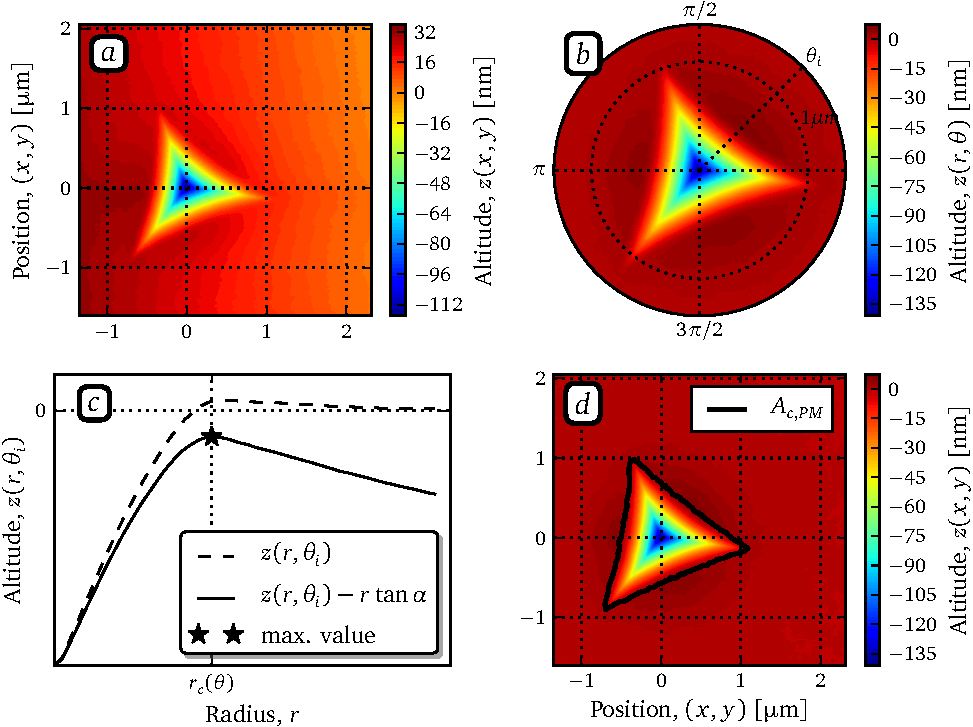
\includegraphics[width =  20cm]{figure_4}
%\captionof{figure}{Key steps of the proposed method exemplified on a Berkovich indent performed on window glass with $P_{max} = 10\;mN$. (\textbf{a}) Raw ITSPM image on which the tilt has to be corrected using a linear least squares fit on each individual scan with a circular mask around the indented region. (\textbf{b}) An half cross section at a given angle $\theta_i$ is extracted. (\textbf{c}) The half cross section $z(r, \theta_i)$ is rotated by a tilt angle $\alpha = 2.5$\degr~ in order to isolate more efficiently the edge of the contact zone. (\textbf{d}) The process is repeated for all required values of $\theta_i$ and the whole contact zone is extracted (in black).}
%
%\end{center}
%
%
%
%
%\begin{center}
%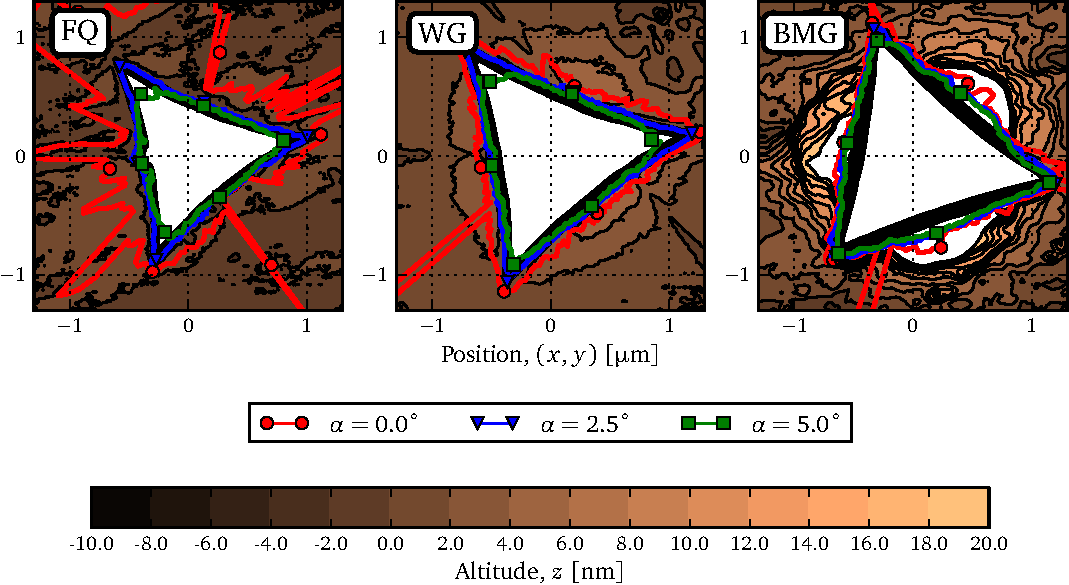
\includegraphics[width =  20cm]{figure_8}
%\captionof{figure}{\textcolor{blue}{Contact contours produced by the proposed method on the three residual imprints measured on each samples composing the benchmark. The imprints were produced using the experimental protocol described in the section \ref{subsec:expe_testing} and the Fig. \ref{fig:figure_3}. Three values of the tilt angle $\alpha$ are investigated on each imprint: no tilt ($\alpha = 0$\degr), the proposed value ($\alpha = 2.5$\degr) and last higher one ($\alpha = 5$\degr).}}
%\end{center}
%
%
%
%
%
%\begin{center}
%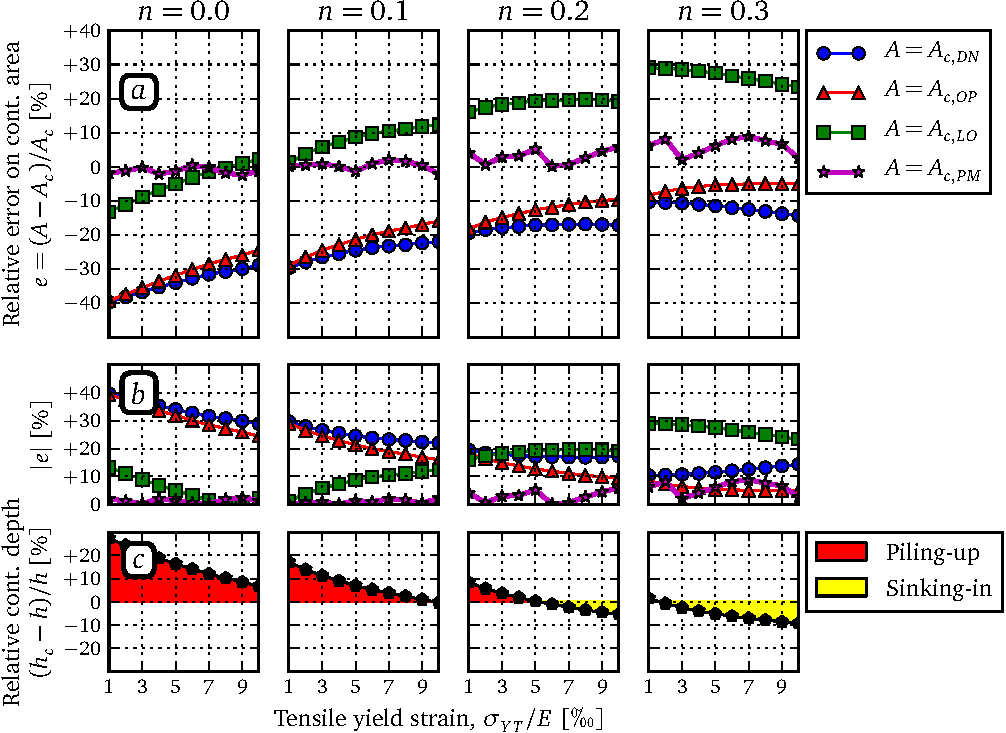
\includegraphics[width =  20cm]{figure_5}
%\captionof{figure}{Benchmark results of three direct methods and of the Proposed Method (PM) in the case of CE1. Different combinations of the tensile yield strain $\sigma_{YT}/E$ and the hardening exponent $n$ are investigated (see Table \ref{tab:hollomon_params}). On each simulation, the true projected contact area ($A_c$) computed by FEM, the contact areas estimated from the three direct methods ($A_{c,DN}$, $A_{c,OP}$ and $A_{c,LO}$) and the contact area from the proposed method ($A_{c,PM}$) are calculated. (\textbf{a}) The relative error $e$ between the true projected contact area and its four estimations is plotted. Each plot represents a different value of the hardening exponent $n$. (\textbf{b}) The absolute value of the the relative error $|e|$ is represented in order to emphasize the accuracy of each method (see Table \ref{tab:num_bench}). (\textbf{c}) The contact depth $h_c$ stands for the axial distance between the edge of the contact zone and the the summit of the indenter. The relative difference between the contact depth and the penetration $h$ is plotted to indicate where the piling-up occurs ($(h_c-h)/h > 0$) and when sinking-in occurs ($(h_c-h)/h < 0$). This subplot helps in understanding the relationships between the occurrence of piling-up and the accuracy of a given method.}
%\end{center}
%
%
%
%
%\begin{center}
%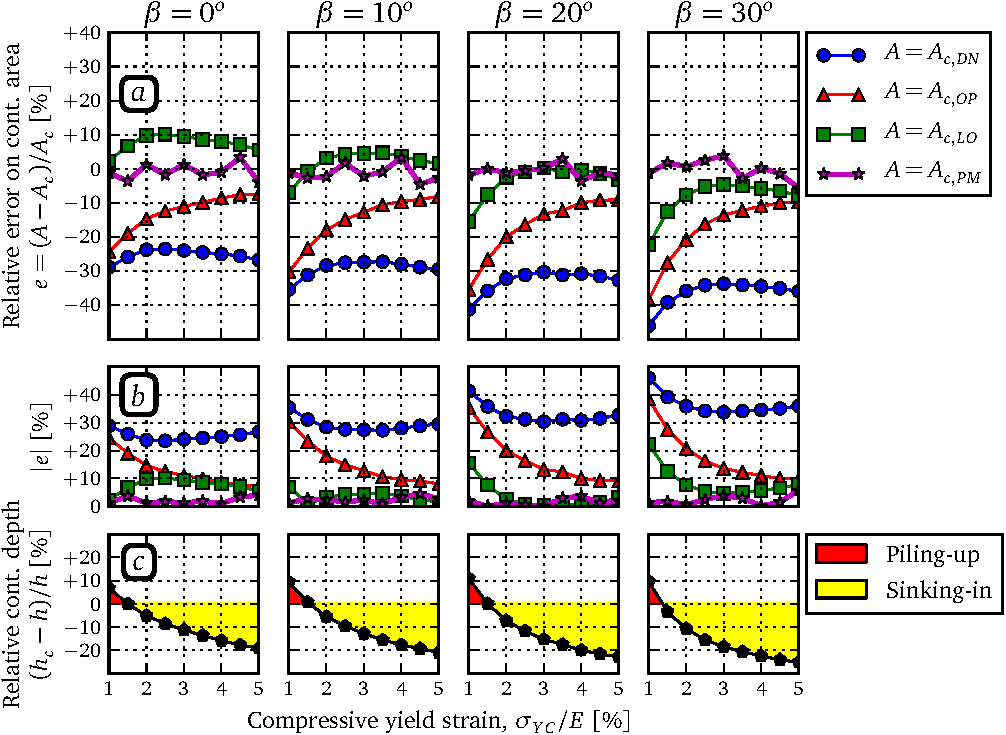
\includegraphics[width =  20cm]{figure_6}
%\captionof{figure}{Benchmark results of 3 direct methods and of the Proposed Method (PM) in the case of CE2. See Figure \ref{fig:figure_5} for the complete description of the structure of the figure.}
%
%\end{center}
%
%
%
%\begin{center}
%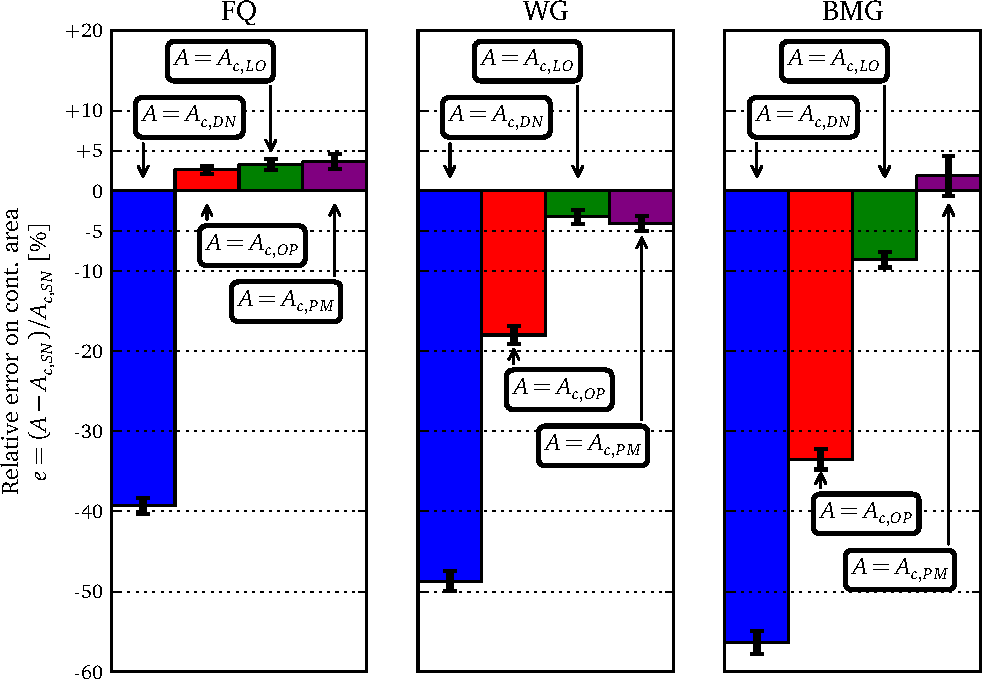
\includegraphics[width =  20cm]{figure_7}
%\captionof{figure}{Experimental confrontation of the three direct methods and the Proposed Method (PM) on the experimental benchmark. The relative error between the true projected contact area computed by Eq. \ref{eq:sneddon} and each method is plotted. Each subplot is dedicated to one sample and each bar within each plot refers to one of the four methods. The error bars represent the standard deviation obtained for four tests performed on each samples.}
%\end{center}
%
%
%%----------------------------------------------------------------------------------------
%%	GEOLOGY
%%----------------------------------------------------------------------------------------
%
%
% %----------------------------------------------------------------------------------------
%%	REFERENCES
%%----------------------------------------------------------------------------------------
%
%\nocite{*} % Print all references regardless of whether they were cited in the poster or not
%\bibliographystyle{plain} % Plain referencing style
%\bibliography{sample} % Use the example bibliography file sample.bib
%
%%----------------------------------------------------------------------------------------
%
%\end{multicols}
\end{document}